\chapter{New and emerging methods and opportunities}\label{sec:emerging-methods-opportunities}

Statewide modeling is on the brink of a dramatic revolution. It has gone from being employed in only a few dozen states a decade or two ago to use in almost all states. They are being used to inform a wide variety of policy and investment decisions, and are becoming more mainstream in statewide and regional planning processes. The experience gained with a wide variety of approaches, and varying degrees of resolution and sophistication, is slowly resulting in a standard practice of statewide modeling. However, there are several important methodological and technical trends that are quietly reshaping how statewide models are built and used, as well as how they evolve and are used to communicate results to a wider audience than modelers:

\begin{itemize}
\item Vastly expanded use of big data to build networks, trip matrices, and eventually, travel diaries for both personal and commercial travel
\item Incorporation of national data and models in place of current long-distance travel models, particularly for visitors
\item The potential for using networks and time series of travel times from person and commercial vehicle navigation system
\end{itemize}

These influential trends are described in this chapter. Some are mature enough for immediate implementation, while others are emerging Individually they can substantially improve statewide models at a reasonable cost, but even more so collectively. How big data might be used to develop and maintain statewide models are discussed next, followed by a discussion about how national models might usefully inform statewide models and reduce the amount of work required to represent external and national markets. Strategic visioning models might also have a place in statewide modeling, either alone or in combination with more traditional approaches, as discussed next. The potential for using the same networks used in personal and in-vehicle navigation systems are discussed next. The chapter closes with a brief discussion about how states might jointly develop and maintain models, reducing the cost to each.

\section{The potential of big data}

Transportation planners have high expectations about the utility for and low cost of big data in all aspects of their work. Statewide modelers have the same expectations, and have already begun to use them in several cases, as described in \S\ref{sec:nontraditional-person} (for person travel models) and \S\ref{sec:nontraditional-freight} (for freight applications). These data can provide information about infrequent long-distance trips by residents of the study area, as well as detailed data about the travel patterns of visitors within it. At present these data are normally supplied in traditional trip matrices for person travel, with rather coarse trip purpose definitions, and their more successful uses appear to be with larger zone sizes. Some vendors offer similarly aggregated travel time information. By themselves, these data only inform us about past travel patterns, but provide no insight into the characteristics of the traveler or trip, or their interactions. They also provide no insight into how trips are structured into tours to meet the full travel needs of an individual or household.

Many believe that this represents the first successful use of big data in travel demand modeling. They are correct about the sheer volume of data, for just storing a few years of the raw cellular tracking data used to build these data for a single state or metropolitan area requires petabytes of data storage. Mining these data requires formidable computing resources and talent, which none of the states have developed or revealed plans to. However, the USDOT has already invested in big data compared to the traditional practice of travel demand modeling over the past few decades. The NHTS represents a significant national resource, even if its sample size in any one given metropolitan area or state precludes it from being used alone to build robust models. The CFS and FAF, discussed in \S\ref{sec:traditional-freight-data}, were not designed as big data programs, but arguably have become so.

As noted, these data can immediately be used to build trip matrices that can be used as calibration and validation targets for trip distribution or destination choice models. The behavioral insights offered through estimation of destination choice models, for example, provide insight into the variables most influential in traveler decision-making. However, the household travel surveys used to develop such models lack enough observations to enable the analyst to ensure that the spatial patterns of destinations chosen, which are unique for each modeled area, are replicated to an acceptable degree. We have a lot to learn about how to combine small household travel surveys with data from tracking half of the population through time and space within the modeled area, but the resulting models will be remarkably more robust than those employed today. Several states, including North Carolina and Ontario (Canada) are known to be experimenting with such techniques.

The vast potential for third-party and government big data programs will emerge when methods for fusing them mature. The raw GPS tracking data can be associated with surrounding land use information at stop locations, and perhaps focused analyses of large clusters of activities. More powerful would be analyses of patterns of joint or similar travel behaviors. However, such matching will likely always be ambiguous except in cases of stops at isolated facilities, or large campuses (e.g., schools and universities, medical centers, factories).

A more expansive approach is to fuse both actively and passively collected data using new methods. \cite{kressner16} created tour patterns for medium-sized communities from fusing the tour patterns found in the NHTS with AirSage origin-destination matrices, using discrete event simulation (DES). The resulting tours from the prototype model replicated observed flows on the Asheville, NC network as well as a well-calibrated trip-based model. This type of DES has not previously been used in travel demand forecasting. However, it has been widely used in other domains to replicate individuals and systems using data collected at varying levels of spatial, temporal, and behavioral resolution. Such models often use a variety of modeling approaches within each modeling system, to include deterministic and stochastic models, sampling from observed or asserted distributions, rule-based methods, and evolutionary models. Artificial intelligence approaches, such as neural networks, might also be employed. The point is that several alternatives to deterministic discrete choice models based on econometric estimation abound, many of which are much better suited for DES and other approaches to fusing, mining, and forecasting with big data.

\section{Integration with national models}\label{sec:national-model-integration}

Statewide modelers a generation ago were faced not only with the challenge of building models capable of capturing the diversity of travel within their state, but to also account for trade and travel with others states and through trips (i.e., trips with both ends outside of the modeled area). In some cases, flows on Interstate highways in adjacent states affect those within the modeled area, but little is known about who travels on them or why. The auto industry in Michigan, for example, had supply chain linkages all over the continent, with different mode choice possibilities depending upon the commodity and distance traveled to or from the state. Their statewide modelers were faced with the need to represent external markets (outside the state), as well as estimating flows to and from them. Commodity flow models were often developed using the CFS, often duplicating the work in nearby states, or expending considerable efforts of their own.

The FAF changed that, such that many states now use the FAF or Transearch data (described in \S\ref{sec:traditional-freight-data}) in conjunction with a scaled-back version of a national network, such as the Oak Ridge Network. Such models can be developed quickly, and in a consistent manner, from well-documented public data. It lacks the level of geographic detail required for most statewide models, but a wide variety of techniques exist for imputing more detailed origins and destinations. As noted earlier, the ATRI truck GPS tracking data are already being widely used for synthesizing long-distance truck origins and destinations at the statewide model zone system. This practice will become the norm in statewide modeling, if not already so in many states. Moreover, the GPS tracking data can be used to check and adjust the FAF flows for individual states in ways that are not yet available at the national level.

One criticism of the FAF is that it is an inventory of existing flows, with static (policy-in\-sen\-si\-tive) forecasts for future years. This limitation is being addressed through the development of a be\-hav\-iorally-based national freight demand model. It is currently under development by FHWA, and expected to include explicit models of freight generation, destination, and mode choice within a supply chain perspective, as well as truck tour formation and routing heuristics. The model is based on a newly proposed national use model areas (NUMA), consisting of counties across the country and further disaggregated into Public Use Microdata Areas (PUMA) within the more populous ones. This will provide at least an order of magnitude more geographic specificity than the FAF data. Combined with truck GPS data to illuminate clusters of truck activities within each zone, this national model will surpass the capabilities of almost all statewide freight models in existence. This will enable states to "plug-and-play" with the national model, reducing the cost and development time associated with building customized models for each state. The funding formerly associated with the latter can presumably be pooled to improve the extent and quality of data used in the national model, enabling it to improve in quality as it evolves, much as the FAF has done.

A similar framework has been proposed for a national long-distance person travel model \citep{outwater14}. The proposed modeling system consists of a tour-based microsimulation of annual long-distance person trips for all travel purposes and modes of transportation. It is conceptually more sophisticated than a similar simulation developed by \cite{moeckel11}, which only replicates existing patterns. The design proposed in this research includes activity participation and scheduling, time use, and joint mode and destination choice models at the level of the same 4,570 NUMAs proposed for the national freight model. A proof of concept was developed, although as research conducted under USDOT's Exploratory Advanced Research program rather than as an ongoing federal effort. It will require major new data collection on long-distance travel on a national scale to succeed. These requirements are well beyond the data available from the long-distance NHTS described in \S\ref{sec:traditional-person}, even if supplemented with similar surveys from states that have conducted them recently, such as California and Ohio. It is presumed that the long-distance element of the more recent California Household Travel Survey would be included as well.

The development and maintenance of a statewide model would be considerably simplified by incorporating these two national models. Ideally, both would be based upon the same NUMAs and national network, and use consistent land use, socioeconomic, and transportation system assumptions and data. There are several challenges associated with such an approach, to include the interface between the more detailed statewide geographic and network coverages used at the statewide level. The precision and accuracy of the national models, how the national models would be run within the statewide model, and data interchange between the different modeling systems are also important issues. It is assumed that these integration issues, similar in many ways to the issue of statewide-urban model integration, are details that can be overcome. It remains an open question whether USDOT, or perhaps a coalition of states, will support these national models.

A conceptual view of such an integrated modeling system is shown in Figure \ref{fig:integrated-opportunities}. National multimodal forecasts of long-distance travel can be published for forecast years, in much the same way the FAF is disseminated. In an ideal configuration, the states could make custom runs of the national model, to explore how changes in assumptions about socioeconomic and transportation system growth might affect long-distance travel patterns. In either case, the data can be accepted by the statewide model, and allocated to finer temporal and geographic representations if required. The data used to build and apply the national models could also be accessed directly by statewide modelers.

\begin{figure}[!t]   % 41
\centering
% Change scale when found
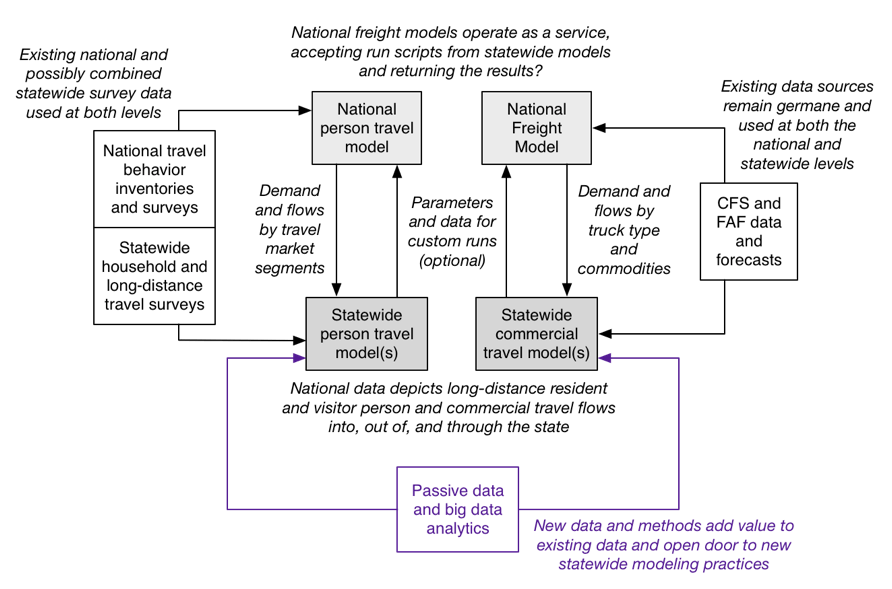
\includegraphics[width=6.5in]{graphics/41-integrated-modeling-opportunities}  
\caption{A vision of integrated statewide-national modeling opportunities}
\label{fig:integrated-opportunities}
\end{figure}

Such a system is neither far-fetched nor fanciful. Such capabilities have long been sought by statewide modelers, and it is thought that such models could place the state within its national context. Perhaps more importantly, it would substantially reduce the costs borne by the states for each to mimic such capabilities.

\section{Strategic visioning models}\label{sec:strategic-visioning-models}

While a standard practice of statewide modeling has yet to emerge, it is safe to assert that most are built using the traditional trip-based modeling paradigm, with flows assigned to a statewide or regional transportation network. In a few cases, states and researchers have experimented with lightweight scenario evaluation models over the past decade, and have found them to be useful adjuncts to the models described in this report. Such models are often described as sketch planning, scenario evaluation, or strategic planning models.

One visioning model designed for statewide modeling was developed by the Oregon DOT. They developed their GreenSTEP model in-house to quickly assess a wide range of potential greenhouse gas emission reduction strategies. The model starts by generating synthetic households across the state. Typical travel patterns mined from the NHTS are applied to households, based upon their characteristics. Aggregate measures of travel are obtained, such as vehicle miles and hours of travel per household. Finally, greenhouse gas emission calculations are carried out to characterize Oregon's footprint.

Mobile emissions of greenhouse gasses are not as influenced by vehicle operating cycle as other emissions, so a simpler congestion model is used to allocate VMT to speed bins. This obviates the need for a detailed network model to obtain accurate estimates. Moreover, the results are compared to statewide reduction targets, reducing the need for the higher levels of spatial, temporal, and behavioral resolution found in current statewide models. Because of the focus on greenhouse gas emissions, the model pays much more attention to vehicle and fuel characteristics than do traditional travel demand models.

A key advantage to using GreenSTEP is its ability to very rapidly assess many alternate futures. Changes in demographics can be easily handled, and the analyst can also change the distributions and rates obtained from the NHTS to evaluate the extent to which current choices would have to change to meet Oregon's greenhouse gas reduction targets. Although applied at the state level, households could be segregated by planning region or metropolitan area to examine outcomes by sub-state areas.

Several variants of GreenSTEP have been developed, including ODOT's Regional Strategic Planning Model (RSPM), FHWA's Energy and Emissions Reduction Policy Analysis Tool (EER\-PAT), and AASHTO's Rapid Policy Analysis Tool (RPAT). An effort is now underway to refactor these models in the new VisionEval model system and software framework to enable model components to be more easily shared between models and to enable the model system to be more easily expanded with new components.

What has not yet happened is tighter integration with mainstream models. Such could be accomplished through the linkages illustrated in Figure \ref{fig:visioneval-swim}. Note that this concept and illustration are ideas of the author, not part of the Oregon Modeling Improvement Program or official plan. Selected scenarios from a VisionEval model could be pushed to the statewide model for closer study, while the more detailed travel characteristics from the statewide model, estimated from their statewide household travel survey, could be used in place of the more generic NHTS estimates of travel behavior. The benefits of using both types of models together seem likely to exceed the value of either alone, and is proposed as an opportunity for expanding the tools available to statewide modelers.

\begin{figure}
\centering
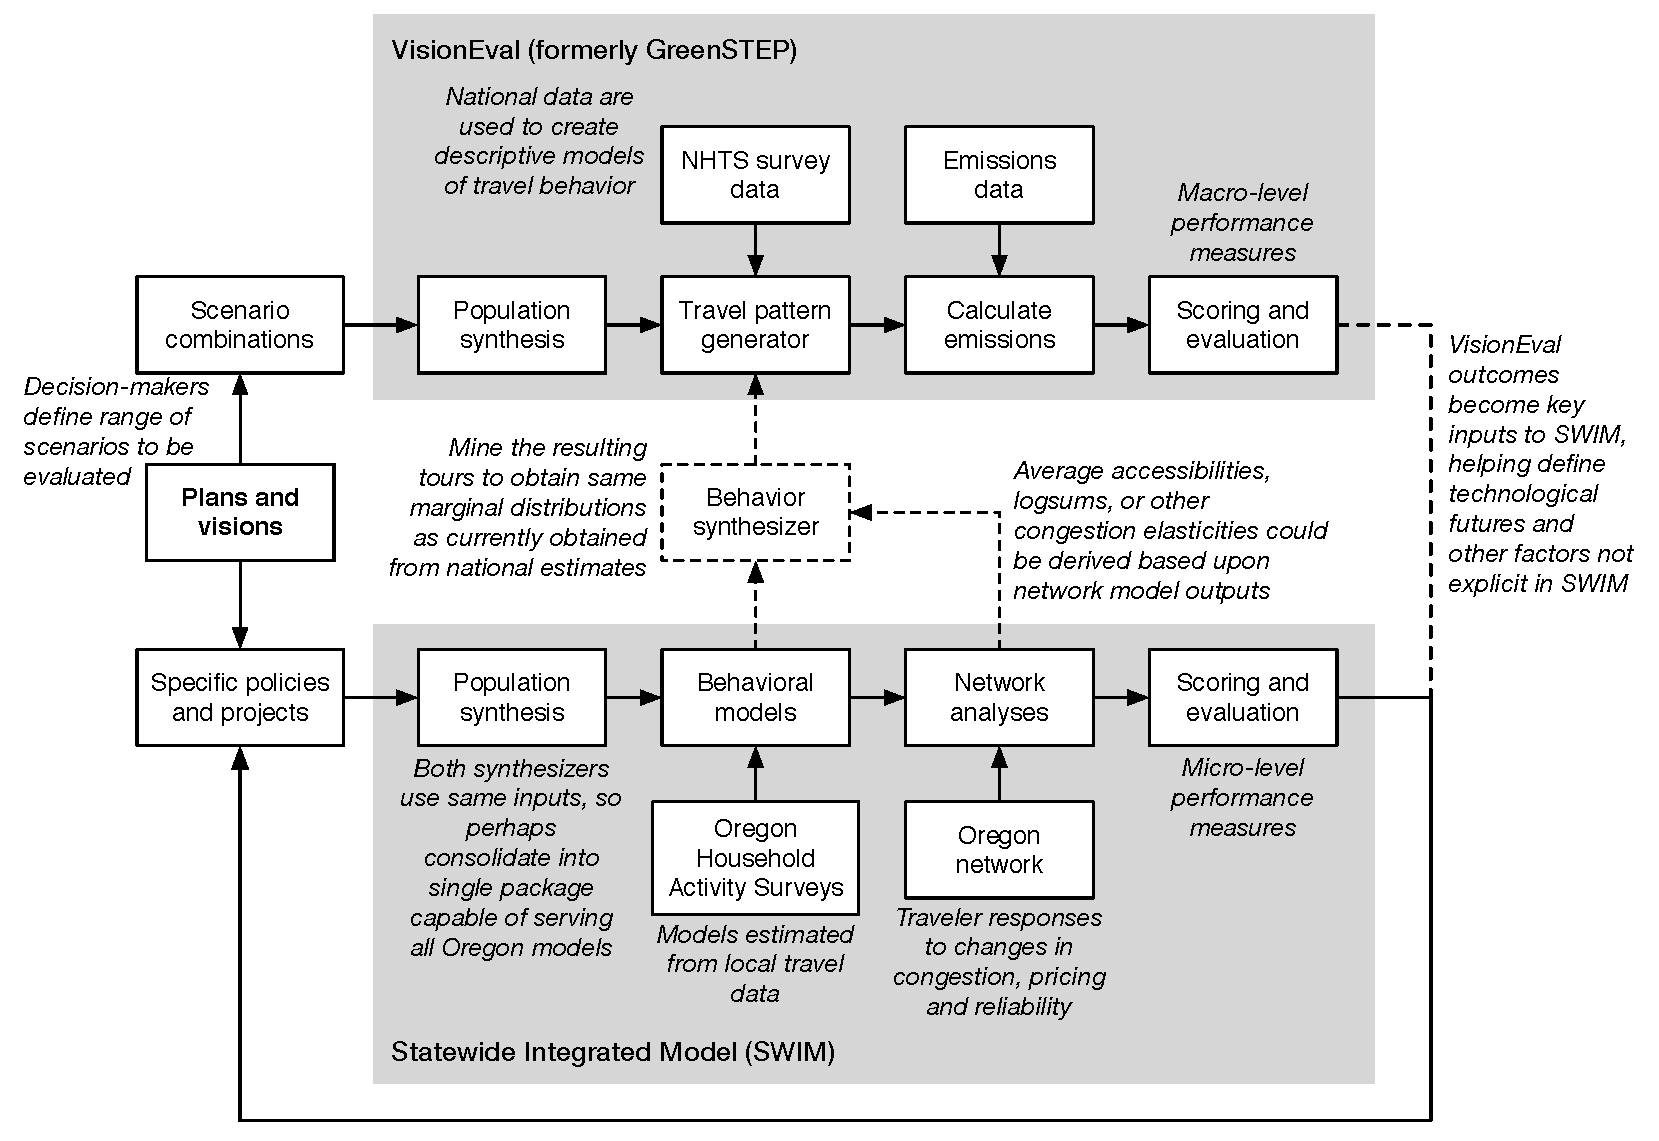
\includegraphics[width=6.5in]{graphics/42-visioneval-swim-integration}
\caption{Hypothetical framework for unifying Oregon visioning and statewide models}
\label{fig:visioneval-swim}
\end{figure}

\section{Navigable networks}

The development of most statewide model networks is an expensive and ad hoc process. It is reported to be among the most onerous parts of statewide modeling, as noted in \S\ref{sec:network-representations}. None of these take advantage of the routable networks used for personal and vehicular navigation systems. While none of the various technology companies that provide such systems, such as Google, Waze, and Apple are known to share their network information, a great deal of interest was expressed by model developers to use them. There are formidable obstacles associated with doing so, to include the likely licensing terms and cost involved. The former may restrict usage of the data to periods when licensing or subscription is in effect, and the annual costs might be much higher than the one-time investment made in most statewide networks. Moreover, the networks themselves lack many of the attributes used in traditional traffic assignment methods. Some might easily be imputed, but others, such as functional classification, might require conflation of navigable networks and traditional network line layers.

If navigable networks became available, they would invite us to rethink how we carry out network analyses in all types of transport models. Widely-used macroscopic assignment models yield closed-form solutions even in hyper-congested states, but are sensitive to assumptions about the relationship between congestion and travel time (expressed as link capacity functions) and link attributes that are often coded by functional classification of the link. Navigation systems find time-dependent optimal routes through congested networks without knowing most of that information. Moreover, such systems have a history of observed travel times that can be flexibly defined by the analyst (e.g., hourly, variations by week). Such information cannot be known for facilities or services that do not exist or might be substantially different in the future. However, in systems where new infrastructure is being built less frequently such data-driven routing heuristics might become a viable alternative to current traffic assignment models.

Dynamic network models are also increasing in popularity, and several researchers have investigated their suitability for statewide modeling. \cite{erdogan14} investigated the use of dynamic traffic assignment (DTA) in Maryland, using a prototype version in TRANSIMS. It was thought that DTA would provide a better estimate of travel times experienced by travelers in the highly-congested Baltimore-Washington corridor. MATSim has been used for network analyses in several national models in Europe, most successfully in Germany. Several of our survey respondents ranked DTA as high on their list of desired model enhancements. Planning-level DTA procedures, which use essentially the same node-abstract representation of roadways as do macroscopic models, seem ideally suited to the task. This obviates the need to represent traffic signals across the state explicitly, which would be a Herculean task for most states to code or maintain timing plans for.

Activity-based models, now used in many major metropolitan areas, are often based on microsimulated households whose full attributes are carried through the simulation. No information is lost along the way, enabling flexible and sophisticated data mining of model results and detailed analyses of market segments. The same approach is gaining traction within statewide modeling. In essence, activity-based models synthesize a travel diary for each simulated person and household. Individual vehicles in dynamic network models can be associated with these diaries, enabling the modeler to better understand the population using a specific facility, an hour of the day, or other grouping variables.

\section{Multi-state models}

Many of the models we reviewed incorporated parts of adjacent states, some of which had almost as much detail as the statewide model in that state. Urban areas beyond the state border, especially when they are agglomerations, heavily influence both person and freight traffic patterns. The ability to bring the effect of important nearby markets into the model was one of the driving motivations for building the Chesapeake megaregional model. The benefits obtained from doing so were clear. There has been surprisingly little interest in consolidating resources by building multi-state or megaregional models, despite the apparent benefits. Several reasons were cited for this:

\begin{itemize}
\item Lack of control over model design, development priorities, or delivery deadlines
\item Increased effort required to run the model, owing to increase coordination with and data supplied by other states involved
\item Unique analytical requirements that other states do not have
\item Desire to retain capability to quickly adapt or change the model if required to meet new analytical requirements
\end{itemize}

These requirements appear to outweigh the potential for cost and data-sharing, and ability to satisfy common goals for model functionality and elimination of boundary effects at state borders. Moreover, computational and institutional issues will need to be overcome before multi-state models emerge in practice.
